\documentclass[twoside]{article}

\usepackage[math]{kurier}
\usepackage[sc]{mathpazo}
\usepackage{amsmath}
\usepackage[T1]{fontenc}
\renewcommand{\sfdefault}{kurier}


\usepackage{graphics}
\setlength{\oddsidemargin}{0.25 in}
\setlength{\evensidemargin}{-0.25 in}
\setlength{\topmargin}{-0.6 in}
\setlength{\textwidth}{6.5 in}
\setlength{\textheight}{8.5 in}
\setlength{\headsep}{0.75 in}
\setlength{\parindent}{0 in}
\setlength{\parskip}{0.1 in}


\newcounter{lecnum}
\renewcommand{\thepage}{\thelecnum-\arabic{page}}
\renewcommand{\thesection}{\thelecnum.\arabic{section}}
\renewcommand{\theequation}{\thelecnum.\arabic{equation}}
\renewcommand{\thefigure}{\thelecnum.\arabic{figure}}
\renewcommand{\thetable}{\thelecnum.\arabic{table}}


\newcommand{\lecture}[3]{
   \pagestyle{myheadings}
   \thispagestyle{plain}
   \newpage
   \setcounter{lecnum}{#1}
   \setcounter{page}{1}
   \noindent
   \begin{center}
   \framebox{
      \vbox{\vspace{2mm}
    \hbox to 6.28in { {\bf \sffamily AA 274: Principles of Robotic Autonomy
                        \hfill Winter 2019} }
       \vspace{4mm}
       \hbox to 6.28in { {\sffamily{\Large \hfill Lecture #1: #2  \hfill}} }
       \vspace{2mm}
       % \hbox to 6.28in { {\it \hfill Scribes: #4} }
      \vspace{2mm}}
   }
   \end{center}
   \markboth{Lecture #1: #2}{Lecture #1: #2}

   \vspace*{4mm}
}

\usepackage{graphicx}

%%%%%%%%%%%%%%%%%%%%%%%%%%
%document
\begin{document}
%modify this
\lecture{3}{Open-Loop and Closed-Loop Motion Control}{}
\section{Introduction}

This lecture discusses the main techniques in optimal control and trajectory optimization.

First, we will review constrained optimization by formulating the problem using the Lagrangian. Then we will explore two different methods in solving an optimal control problem: we will thoroughly explore some equations behind Indirect Methods, enabling its computation along with examples, and give an overview on another approach: Direct Methods.
Then we will explore differentially flat problems, and how these enable the use of algebraic equations in non-linear problem solving.
Next we will explore closed-loop control, and some implementations.
Finally, we will combine open-loop and closed-loop approaches by introducing trajectory tracking.

\section{Constrained Optimization}
Before presenting the optimal control problem it is first useful to briefly review a standard constrained optimization problem given by

\begin{equation} \label{const}
\begin{split}
\underset{u}{\text{min}} \:\: &f(x) \\
\text{subject to} \:\: &h_i(x) = 0, \quad i = 1,\dots,m \\
\end{split}
\end{equation}

Problem \ref{const} is solved by introducing the \textit{\textbf{Lagrangian}} and then generating the necessary conditions for optimality (NOC). The Lagrangian is given by

$$L(x,\lambda) = f(x) + \sum_{i=1}^{m}\lambda_i h_i(x)$$

and the necessary conditions for optimality are

\begin{equation} \label{noc}
\begin{split}
\nabla_x L(x^*,\lambda^*) &= 0 \\
\nabla_\lambda L(x^*,\lambda^*) &= 0 \\
\end{split}
\end{equation}

One way to think about the necessary conditions (Eq. \ref{noc}) for optimality is as a filter that takes in all points $x$ and outputs a subset of potential optimal points $x^*$. If several potential points exist that satisfy the NOC, these could be local optima.

\section{Optimal Control Problem}

\begin{equation} \label{optcont}
\begin{split}
\underset{u}{\text{min}} \:\: &h(x(t_f),t_f) + \int_{t_0}^{t_f} g(x(t),u(t),t) dt \\
\text{subject to} \:\: &\dot{x}(t) = a(x(t),u(t),t) \\
&x(t) \in \mathcal{X}, \quad u(t) \in \mathcal{U}
\end{split}
\end{equation}

In general, $x(t) \in \mathbb{•}{R}^n$, $u(t) \in \mathbb{R}^m$, and the initial condition $x(0) = x_0$ is given. In the context of this course the constraint $x(t) \in \mathcal{X}$ is typically relaxed to just be $x(t) \in \mathbb{R}^n$. In other words there are no state constraints.

The problem given by Eq. \ref{optcont} contains many details. In the objective function, the term $h(x(t_f),t_f)$ represents a cost associated with the end condition. For example if you wanted to minimize time you could have $h = t_f$. Also in the objective function, the integral produces a path cost, or in other words produces penalties along the way from $t_0$ to $t_f$. This would be useful if you wanted to minimize fuel use: for example you could set $g = u^2$.

The first constraint in the problem defines the differential constraints that represent the system dynamics. These in general are nonlinear which is why they are represented as $a(x(t),u(t),t)$.

Problem \ref{optcont} is typically solved to yield an open-loop trajectory and control, which are denoted as $x^*(t)$ and $u^*(t)$. Note that these are entire trajectories through time, not just individual points as we saw in Eq. \ref{const}. Since the control is open loop we also typically write

$$u^*(t) = f(x(t_0),t)$$

to indicate that the control is a function of time only, and does not utilize any state feedback.

It is important to realize the difference between solving these optimal control problems and solving general optimization problems. As mentioned, in optimal control we are solving for \textit{trajectories}, and not just points. For any given set of boundary conditions there are an infinite number of possible trajectories, and with the dynamics constraints also involved this becomes a formidable task.

The tools used to solve this Problem \ref{optcont} are generally classified as \textit{\textbf{Indirect Methods}} and \textit{\textbf{Direct Methods}}.



\subsection{Indirect Methods}
%--------------------------Example of Indirect Methods--------------------------%

Given the control inputs and thus the control function (either an open loop or closed loop scenario) we look to optimize over, one can proceed with either a direct or indirect method for solving. A good thought process to follow for an indirect method is to \textit{\textbf{"first optimize, then discretize"}}. The indirect method works by imposing all NCOs, looking at the optimal functions of time we generated, and then selecting the one that is the best. Take the unconstrained finite dimensional case of a simple function f(x) that we look to optimize over $x \in \mathbb{R}^n$:

$$\underset{x}{\text{min}} \:\: \nabla_f(x) = 0 \\$$

Taking the gradient of my function and looking at those candidates that survive, one can determine which values would optimize their function (looking to minimize for our case). Our parallel infinite dimensional problem takes the solutions from NCOs as differential equations which should then be discretized to solve accordingly.

After a series of complicated derivations to establish an augmented cost function and referring to section \textbf{3.2} on how to generally handle constrained optimization, one can arrive at what is known as the Hamiltonian to solve our functions:

\begin{equation} \label{hamiltonian}
\begin{split}
H := g(x(t), u(t), t) + p^\textbf{T}(t)[a(x(t), u(t), t]
\end{split}
\end{equation}
where the first paranthetical term denotes the running cost, $p^\textbf{T}(t)$ denotes the vector of Lagrange Mutlipliers (one for each individual constraint),and the final term denoting the RHS of the differential equation.
From here we can declare the NCO's that our system requires for optimality:
\begin{equation} \label{hamiltonianNCOs}
\begin{split}
\dot{x}^*(t) &= \frac{\partial{H}}{\partial{p}} = (x^*(t), u^*(t), p^*(t), t)\\
\dot{p}^*(t) &= -\frac{\partial{H}}{\partial{x}} = (x^*(t), u^*(t), p^*(t), t)\\
0 &= \frac{\partial{H}}{\partial{u}} = (x^*(t), u^*(t), p^*(t), t)
\end{split}
\end{equation}

The first equation represents the derivative of the Hamiltonian with respect to your individual Lagrange Multipliers which interestingly enough gives back the kinematic state equations of the robot. The second equation is called the costate of your function - looking to optimize the function over continuous infinite time, the lagrange multipliers become functions of time. The final equation is the optimality condition which is simply the Hamiltonian differiniated with respect to the constraint producing an algebraic equation. This is \textbf{under the assumption that we have no state constraints} which is sufficient for our focus of the class. The tedious part of optimal control is now solving these equations: we have produced 2N optimization variables in $x^*(t)$ and $p^*(t)$ with one M varibale $u^*(t)$ totaling 2N + M variables alongside our 2N differinitable equations and M algebraic equation.

To solve we must impose boundary conditions on our function with respect to the robot's final position and time such that:

\begin{equation} \label{hamiltonianBCs}
\begin{split}
[\frac{\partial{h}}{\partial{x}}(x^*(t_f), t_f - p^*(t_f))]^T\delta{x_f}\ + [H(x^*(t_f), u^*(t_f), p^*(t_f), t_f + \frac{\partial{h}}{\partial{t}}(x^*(t_f), t_f)]\delta{x_f} = 0\\
\end{split}
\end{equation}

which produces four possible solutions to satisfy the equation:

$t_f$ = fixed and $x(t_f)$ = fixed \dots $\delta{t_f}$ = 0 and $\delta{x(t_f)}$ = 0

$$\textbf{BC}: x^*(t_0) = x_0$$
$$x^*(t_f) = x_f$$


$t_f$ = fixed and $x(t_f)$ = free \dots $\delta{t_f}$ = 0 and $\delta{x(t_f)}$ = arbitrary

$$\textbf{BC}: x^*(t_0) = x_0$$
$$[\frac{\partial{h}}{\partial{x}}(x^*(t_f), - p^*(t_f))] = 0$$


$t_f$ = free and $x(t_f)$ = fixed \dots $\delta{t_f}$ = arbitrary and $\delta{x(t_f)}$ = 0

$$\textbf{BC}: x^*(t_0) = x_0$$
$$x^*(t_f) = x_f$$
$$[H(x^*(t_f), u^*(t_f), p^*(t_f), t_f + \frac{\partial{h}}{\partial{t}}(x^*(t_f), t_f)]\delta{x_f} = 0$$



$t_f$ = free and $x(t_f)$ = free \dots $\delta{t_f}$ = arbitrary and $\delta{x(t_f)}$ = arbitrary

$$\textbf{BC}: x^*(t_0) = x_0$$
$$[\frac{\partial{h}}{\partial{x}}(x^*(t_f), - p^*(t_f))] = 0$$
$$[H(x^*(t_f), u^*(t_f), p^*(t_f), t_f + \frac{\partial{h}}{\partial{t}}(x^*(t_f), t_f)]\delta{x_f} = 0$$

The last scenario is what we call a free final time state and introduces an unkown variable to our system of equations making it a set of 2N + M + 1. Think of this as an optimal control problem where we look to minimize the cost of our function at any given final time. We look at a thorough example for clarification.

Let's consider an example of free final time. Consider a point that moves in one dimension. Control input of the system is acceleration of the point. Boundary conditions for positions and velocities at initial and final times are given, but the final time is not fixed.

\begin{equation}\label{ExampleSCAndBC}%State Constraints and Boundary Conditions
\ddot{x} = u, x(0) = 10, \dot{x} = 0, x(t_f) = 0, \dot{x}(t_f) = 0
\end{equation}
\begin{equation}\label{ExampleCostFunction}
J = \frac{1}{2}\alpha t_f^2 + \frac{1}{2} \int_{t_0}^{t_f} bu^2(t) \mathrm{d}t
\end{equation}

Cost function shown in \eqref{ExampleCostFunction} is typical in control problems. The final term in cost function tries to minimize total time to get back to origin, while the stagewise cost attempts to keep acceleration from being too high, which requires a lot of control effort. Analytical solution \eqref{ExampleAnalyticalSolution} of the final time is pretty reasonable. When $b$ increases, penalty on control effort will be more serious, which causes the acceleration to be relatively low and $t_f$ to be longer. When $\alpha$ increases, the final cost term will become dominant, so $t_f$ will become shorter.

\begin{equation}\label{ExampleAnalyticalSolution}
t_f = (1800b/\alpha)^{1/5}
\end{equation}

In order to solve the control problem, firstly we need to define state \textbf{z} and Hamiltonian. From the first equation of \eqref{ExampleSCAndBC} we have two state constraints (in which $x_1 = x$). Thus we have two Lagrange multipliers $p_1$ and $p_2$ correspondingly.

\begin{equation}\label{ExampleSC}%State Constraints
\begin{split}
\dot{x_1} &= x_2 \\
\dot{x_2} &= u
\end{split}
\end{equation}

According to the trick for free final time, we have a dummy state $r$ that is equal to $t_f$ with dynamics $\dot{r} = 0$. So state \textbf{z} has five elements.

\begin{equation}\label{ExampleState}
\textbf{z} = [z_1, z_2, z_3, z_4, z_5] ^T= [x_1^*, x_2^*, p_1^*, p_2^*, r^*]^T
\end{equation}

Then we form Hamiltonian $H$ based on \eqref{ExampleCostFunction} and \eqref{ExampleSC}.

\begin{equation}\label{ExampleH}
H = \frac{1}{2}bu^2 + p_1x_2 + p_2u
\end{equation}

We can get Hamiltonian equations from $H$.

\begin{equation}\label{ExampleHEqs}
\begin{split}
\dot{x}_1^* &= \frac{\partial{H}}{\partial{p_1}}(\textbf{x}^*(t),u^*(t),\textbf{p}^*(t),t)= x_2^* \\
\dot{x}_2^* &= \frac{\partial{H}}{\partial{p_2}}(\textbf{x}^*(t),u^*(t),\textbf{p}^*(t),t)= u^* \\
\dot{p}_1^* &= -\frac{\partial{H}}{\partial{x_1}}(\textbf{x}^*(t),u^*(t),\textbf{p}^*(t),t)= 0 \\
\dot{p}_2^* &= -\frac{\partial{H}}{\partial{x_2}}(\textbf{x}^*(t),u^*(t),\textbf{p}^*(t),t)=-p_1^* \\
0 &= \frac{\partial{H}}{\partial{u}}(\textbf{x}^*(t),u^*(t),\textbf{p}^*(t),t) = bu^* + p_2^*
\end{split}
\end{equation}

Boundary conditions include the original ones and substitution for free $t_f$ and fixed $\textbf{x}(t_f)$ problem.

\begin{equation}\label{ExampleBC1*}
x_1^*(0) = 10, x_2^*(0) = 0, x_1^*(t_f) = 0, x_2^*(t_f) = 0
\end{equation}
\begin{equation}\label{ExampleBC2*}
\begin{split}
H(\textbf{x}^*(t_f), u^*(t_f), \textbf{p}^*(t_f), t_f)+\frac{\partial{h}}{\partial{t}}(\textbf{x}^*(t_f),t_f) = 0 \\
\frac{1}{2}bu^*(t_f)^2 + p_1^*(t_f)x_2^*(t_f)+p_2^*(t_f)u^*(t_f) + \alpha t_f = 0
\end{split}
\end{equation}

When you put $u^* = -\frac{1}{b}p_2^*$ and $x_2^*(t_f) = 0$ into \eqref{ExampleBC2*}, you can get a more clear version of the last boundary equation.

\begin{equation}\label{ExampleBC2*Clear}
-\frac{1}{2b}p_2^*(t_f)^2 + \alpha t_f = 0
\end{equation}

After substitution of $u^* = -\frac{1}{b}p_2^*$ into other Hamiltonian equations in \eqref{ExampleHEqs}, we unify the notation of states to \textbf{z} and rescale time with $\tau = t/t_f$. BVP becomes
\begin{equation}\label{FinalBVP}
\frac{\mathrm{d}\textbf{z}}{\mathrm{d}\tau} = t_f\frac{\mathrm{d}\textbf{z}}{\mathrm{d}t}
= z_5\begin{bmatrix}
    0 & 1 & 0  & 0                & 0 \\
    0 & 0 & 0  & -\frac{1}{b} & 0 \\
    0 & 0 & 0  & 0                & 0 \\
    0 & 0 & -1 & 0                & 0 \\
    0 & 0 & 0  & 0                & 0 \\
\end{bmatrix} \textbf{z}
\end{equation}

After the same operation, BC become

\begin{equation}\label{FinalBC}
\begin{split}
z_1(0) = 10, z_2(0) = 0, z_1(1) &= 0, z_2(1) = 0, \\
-\frac{1}{2b}z_4(1)^2 + \alpha z_5(1) &= 0
\end{split}
\end{equation}

Then we can input these BVP and BC into Python to solve the problem.
%--------------------------End of Example for Indirect Methods--------------------------%

%% ------- WINTER 2019, LECTURE 4 SCRIBES, MAKE YOUR EDITS BELOW THIS LINE -------- %%

\subsection{Direct Methods}
The alternate way for solving these optimal control problems is through use of what is known as a direct method where instead we carry out the reverse process and rather textit{\textbf{"first discretize, then optimize"}}. We take our same infinite time dimensional problem, discretize it into itemized finite dimensional elements, and then optimize those parts known as a nonlinear programming problem (NLP).

As direct methods are not highlighted in great detail for the extent of this course a brief conceptual overview is provided. Interested students are referred to further courses and literature for further exploration. Two main ways for carrying out a direct method can be observed through what is called either the \textbf{Control Parameterization Method} which discretizes the control function over n steps treating the trajectory as continuous or through \textbf{State and Parameterization} which discretizes both the state and control functions.

Several software packages including DIDO, Propt, and GPOPS provide excellent tools for solving with these direct method types.

\section{Differential Flatness}
The concept of differential flatness is particularly useful in controlling certain nonlinear systems, especially when explicit trajectory generation is required.

For example, consider the problem of designing a trajectory for a quadrotor (which is a differentially flat nonlinear system). Without leveraging the flatness property, a trajectory designer would have to compute a trajectory for all $12$ state variables, position ($x$,$y$,$z$), velocity ($\dot{x}$,$\dot{y}$,$\dot{z}$), angles ($\phi$,$\theta$,$\psi$), and angular rates ($\dot{\phi}$,$\dot{\theta}$,$\dot{\psi}$), the 4 control inputs ($u_{1,2,3,4}$), and also make sure these satisfy the differential equations $\bar{\dot{x}} = f(\bar{x},u)$.

When utilizing the concept of differential flatness, it turns out that the flat outputs $\bar{z}$ are just the position ($x$,$y$,$z$) and the yaw angle ($\psi$). Therefore a trajectory designer could design trajectories only for these flat variables, and then algebraically compute the remaining states and controls. Simply put, when a nonlinear system is differentially flat the trajectory designer can plan in the flat output space and then directly map those to the appropriate control inputs without having to worry about violating the dynamics equations for the system!

Mathematically, a non-linear system
\begin{equation}
\dot{x} = f(x,u),
\end{equation}

is differentially flat with flat output $z$ if there exists a function $\alpha$ such that

\begin{equation}
z = \alpha (x,u,\dot{u},\dots,u^{(p)}),
\end{equation}

and such that the solutions to the system $x$ and $u$ can then be written as functions of the flat output $z$ and a finite number of its derivatves

\begin{equation}
\begin{split}
x &= \beta (z,\dot{z},\dots,z^{(q)}) \\
u &= \gamma (z,\dot{z},\dots,z^{(q)}) \\
\end{split}
\end{equation}

From these relations we can also write boundary conditions on the flat outputs that encode the initial and terminal conditions.

\begin{equation} \label{flatbc}
\begin{split}
x(0) &= \beta (z(0),\dot{z(0)},\dots,z^{(q)}(0)) = x_0 \\
x(T) &= \beta (z(T),\dot{z}(T),\dots,z^{(q)}(T)) = x_f \\
\end{split}
\end{equation}

Therefore any trajectory for $z$ that satisfies these boundary conditions can be mapped to a feasible trajectory for the nonlinear system. This means that $z$ can be defined however the designer chooses, but a common choice is by using a set of smooth basis functions $\psi(t)$

\begin{equation} \label{flat}
z(t) = \sum_{i=1}^{N} \alpha_i \psi_i(t), \quad \alpha_i \in \mathbb{R}
\end{equation}

For example, one choice is to use polynomial basis functions $\psi_1(t) = 1$, $\psi_2(t) = t$, $\psi_3(t) = t^2$, and so on. Choosing a set of smooth basis functions leads to representation that is linear in the coefficients $\alpha_i$, and thus can be easily identified algebraically.

Taking derivatives of the representation in Eq. \ref{flat} gives

\begin{equation}
\begin{split}
\dot{z}(t) &= \sum_{i=1}^{N} \alpha_i \dot{\psi_i}(t) \\
&\vdots \\
z^{(q)}(t) &= \sum_{i=1}^{N} \alpha_i \psi_i^{(q)}(t). \\
\end{split}
\end{equation}

Given the initial and final conditions $z(0), \: \dot{z}(0), \: \dots , z^{(q)}(0)$ and $z(T), \: \dot{z}(T), \: \dots , z^{(q)}(T)$ that satisfy the boundary conditions in Eq. \ref{flatbc}, the coefficients $\alpha_i$ can be found by solving (assuming full rank)

\begin{equation}
\begin{bmatrix}
    \psi_1(0) & \psi_2(0) & \dots & \psi_N(0) \\
    \dot{\psi_1}(0) & \dot{\psi_2}(0) & \dots & \dot{\psi_N}(0) \\
    \vdots & \vdots & & \vdots \\
    \psi_1^{(q)}(0) & \psi_2^{(q)}(0) & \dots & \psi_N^{(q)}(0) \\
    \psi_1(T) & \psi_2(T) & \dots & \psi_N(T) \\
    \dot{\psi_1}(T) & \dot{\psi_2}(T) & \dots & \dot{\psi_N}(T) \\
    \vdots & \vdots & & \vdots \\
    \psi_1^{(q)}(T) & \psi_2^{(q)}(T) & \dots & \psi_N^{(q)}(T) \\
\end{bmatrix}
\begin{bmatrix}
    \alpha_1 \\
    \alpha_2 \\
    \vdots \\
    \alpha_N \\
\end{bmatrix} =
\begin{bmatrix}
    z(0) \\
    \dot{z}(0) \\
    \vdots \\
    z^{(q)}(0) \\
    z(T) \\
    \dot{z}(T) \\
    \vdots \\
    z^{(q)}(T) \\
\end{bmatrix}
\end{equation}

To summarize, for differentially flat nonlinear systems, nominal trajectories and control inputs can can be computed in a more computationally efficient way.

\section{Closed-loop Control}
In the case of closed-loop control, the goal is to find
\begin{equation}
u^*(t)=\pi(x(t),t)
\end{equation}
often using two main techniques: Lyapunov analysis, or the Hamilton-Jacobi-Bellman equation and dynamic programming. The extent of these methods can be seen in classes such as AA203, however in this class we will primarily consider examples of these applications.
\subsection{Lyapunov proof for stability}
One type of stability for a system is known as Lyapunov stability. Lyapunov stability gives an indication of stability of a initial condition near a given equilibrium. Formally, this can be given as,
for a autonomous nonlinear dynamical system, given by:
\subsubsection{Theorem}
\begin{equation}
\dot{x} (t)=f(x(t)),   x(0) =x_0
\end{equation}

This system is Lyapunov stable if for any $\epsilon$ $>$ 0, there exists a $\delta = \delta (\epsilon)$ such that if $\vert \vert x(0) - x_e \vert \vert < \delta $ then for every t $\geq$ 0,  $\vert \vert x(t) - x_e \vert \vert < \delta$ where $x_e$ is an equilibrium point. \cite{lyupanovproof}


The implication of this is that we are able to determine the stability of a system with respect to its equilibrium points. Systems that are Lyapunov stable will tend to stay "close to" the equilibrium point if a given initial condition satisfies the theorem. This closeness is defined by $\delta$. The full proof for stability can be found in various sources, such as \cite{ee363notes}.
% ----------------- Polar Coordinates and Example---------------- %
\subsection{Example}
Let's consider a differential drive example for closed-loop control. The differential drive mobile robot has unicycle dynamics, which can be described in $XY\theta$ coordinates as follows.

\begin{equation} \label{xytheta}
\begin{split}
\dot{x}(t) &= V(t) cos(\theta(t)) \\
\dot{y}(t) &= V(t) sin(\theta(t)) \\
\dot{\theta}(t) &= \omega(t)  \\
\end{split}
\end{equation}

\begin{figure}[h]
\centering
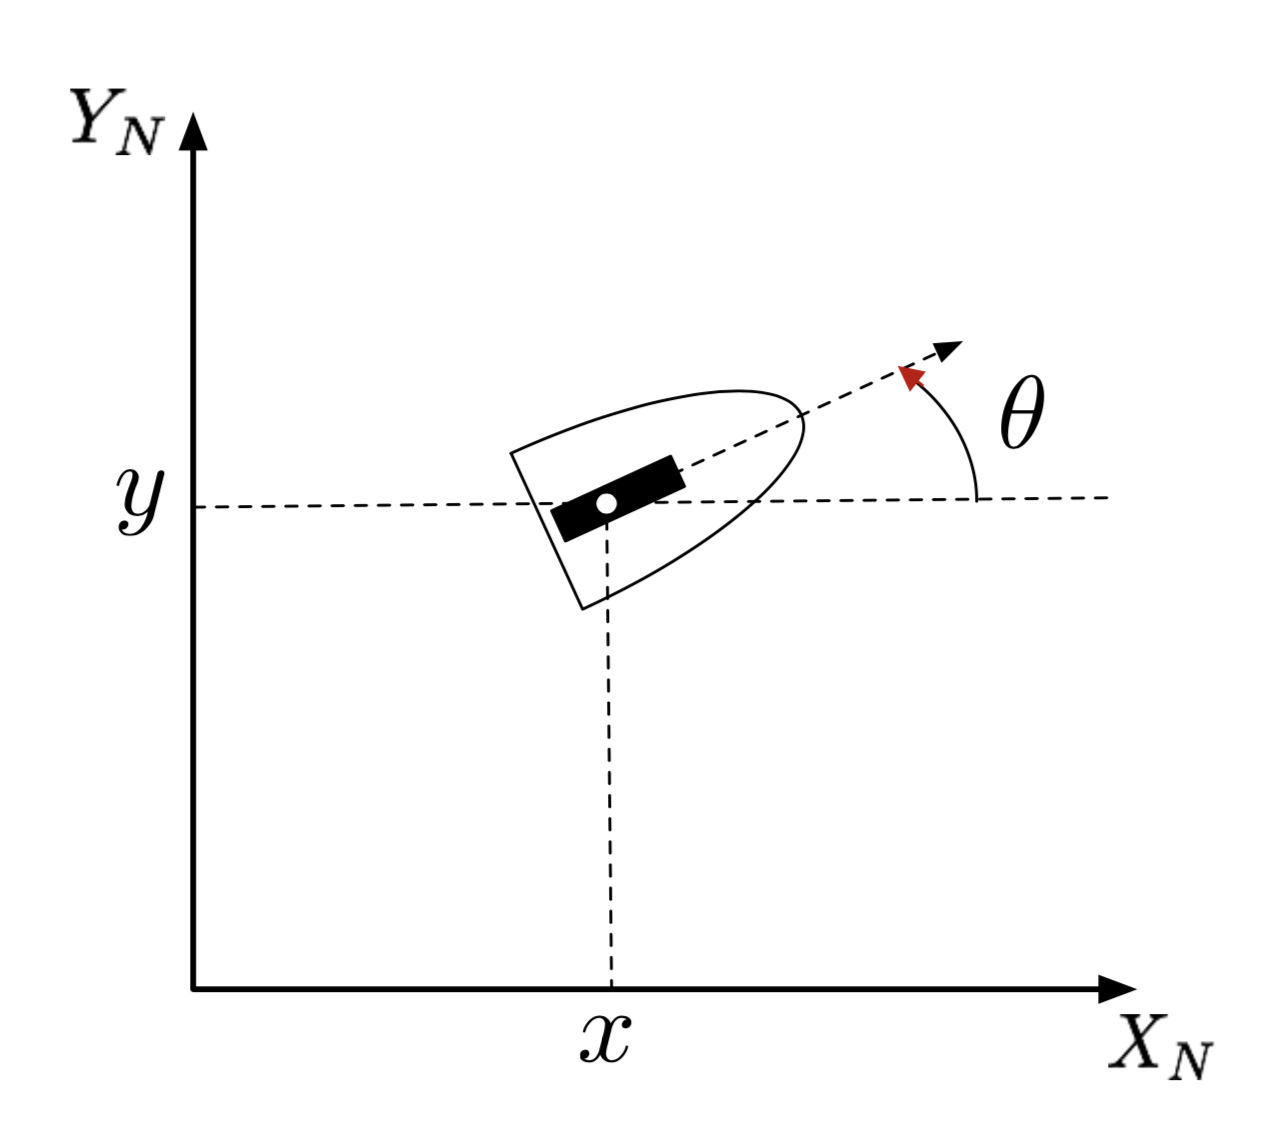
\includegraphics[width=0.5\textwidth]{XYTheta.png}
\caption{$XY\theta$ Coordinates}
\label{XYThetaFigure}
\end{figure}

The control inputs of this system are $V$, which is linear velocity of the wheel and $\omega$, which is angular velocity around the vertical axis. It has been revealed that the system cannot be controlled in a closed loop with continuous time and variant feedback. In particular, if you set control inputs all to zero, the system will be stopped immediately. This feature has some advantages from a control standpoint, but clearly it is not realistic since no dynamical systems can be stopped immediately. However, many systems in real world can be adjusted model of this version.

\subsection{Polar Coordinates}
It is actually easier to design a closed-loop controller based on polar coordinates than $XY\theta$ coordinates. The polar coordinates are established according to desired state of the unicycle. Origin is at the desired position and $X_N$ axis is along the main axis of the robot. The position is defined as center of the rear axis of the vehicle. The main axis is defined as the longitudinal axis of the robot.

We describe states of the robot by polar coordinates $\rho$, $\alpha$ and $\delta$ instead of $X$, $Y$ and $\theta$:
\begin{itemize}
  \item $\rho$: distance of the reference point of the unicycle from the goal
  \item $\alpha$: angle of the pointing vector to the goal with respect to the unicycle main axis
  \item $\delta$: angle of the same pointing vector with respect to the $X_N$ axis
\end{itemize}

\begin{figure}[h]
\centering
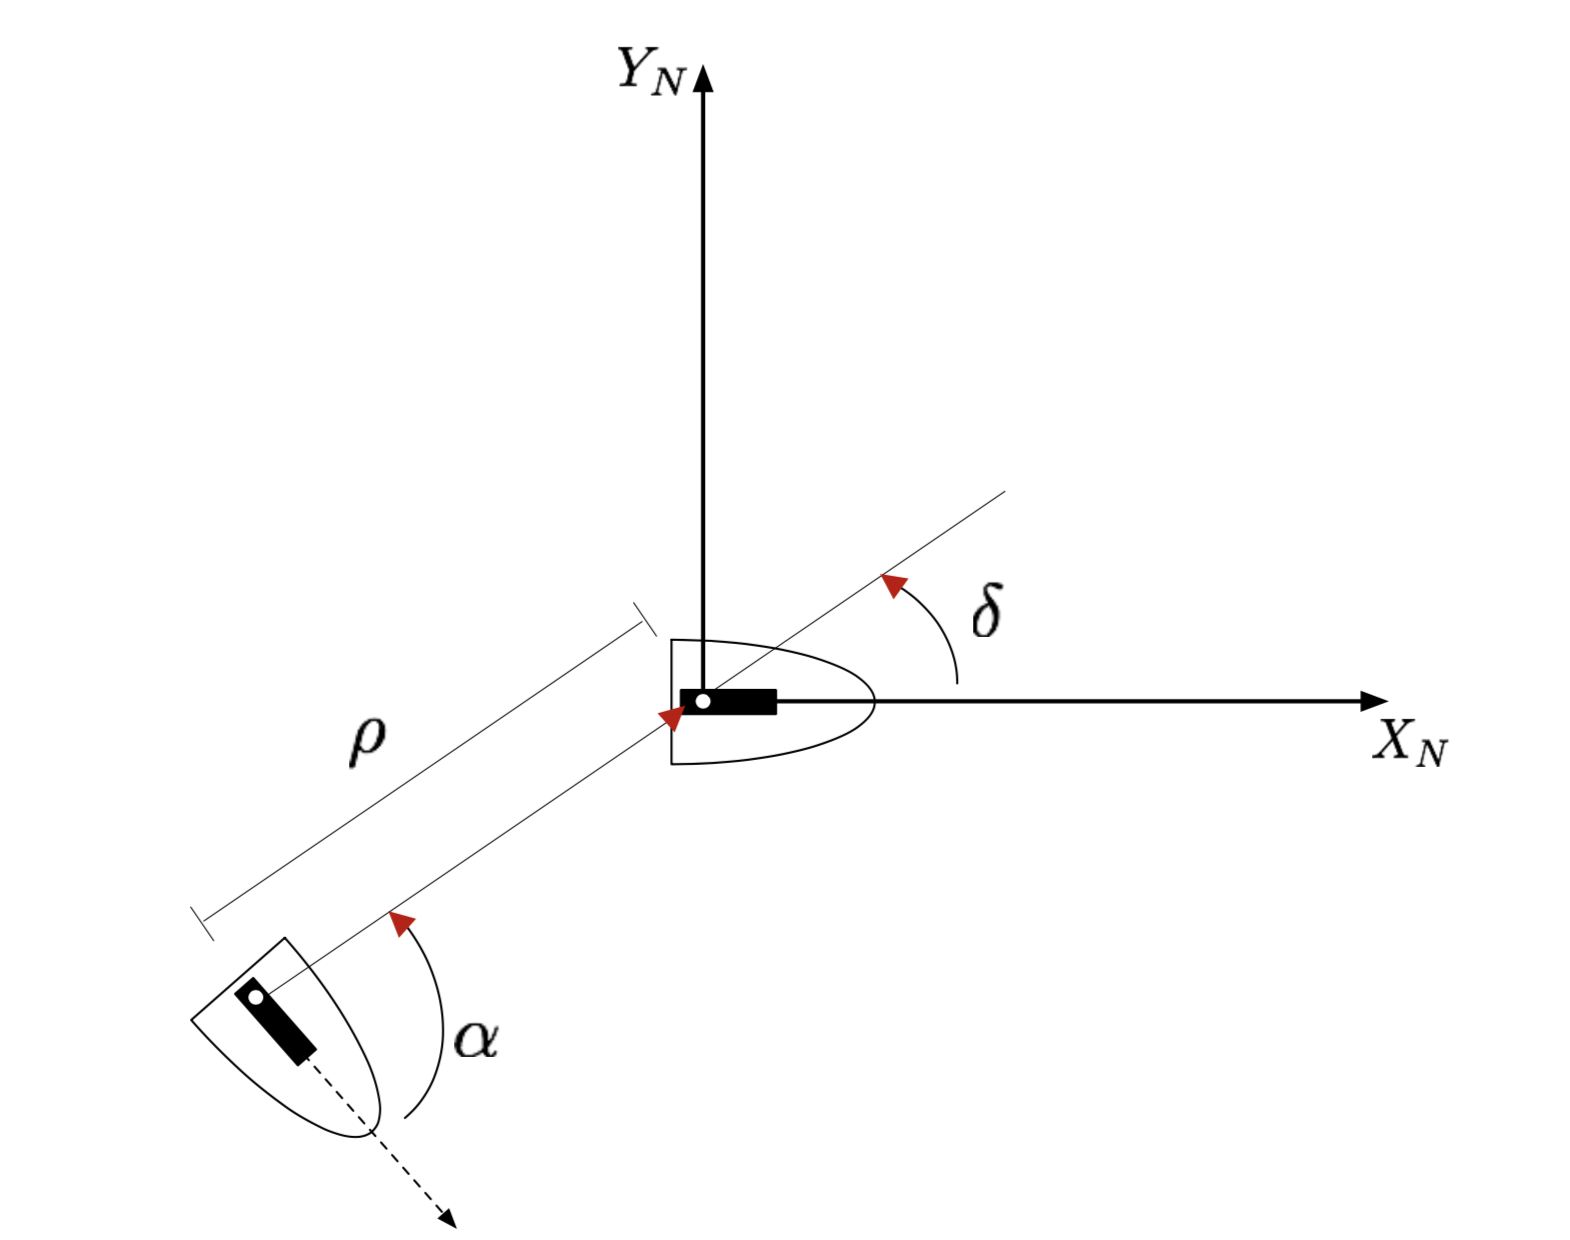
\includegraphics[width=0.5\textwidth]{RhoAlphaDelta.png}
\caption{Polar Coordinates}
\label{RhoAlphaDeltaFigure}
\end{figure}

Coordinate transformation between $\rho\alpha\delta$ and $XY\delta$ coordinates:
\begin{equation} \label{coordinate transformation}
\begin{split}
\rho &= \sqrt{x^2+y^2} \\
\alpha &= \mathrm{atan2}(y, x) - \theta + \pi \\
\delta &= \alpha + \theta \\
\end{split}
\end{equation}

Let's derive dynamic equations of the unicycle in polar coordinates. Say current position of the unicycle is at point $P$ and the origin is at point $O$. $\overrightarrow{OP}$ is position vector of the unicycle. The control input $\omega$ cannot move the position, so $\dot{\rho}$ comes from the other input $V$.

\begin{equation} \label{dotrho}
\begin{split}
\dot{\rho} &= \vec{V} \cdot \overrightarrow{OP}/||\overrightarrow{OP}|| \\
\dot{\rho} &= V \cos(\pi - \alpha) = -V \cos\alpha \\
\end{split}
\end{equation}

\begin{figure}[h]
\centering
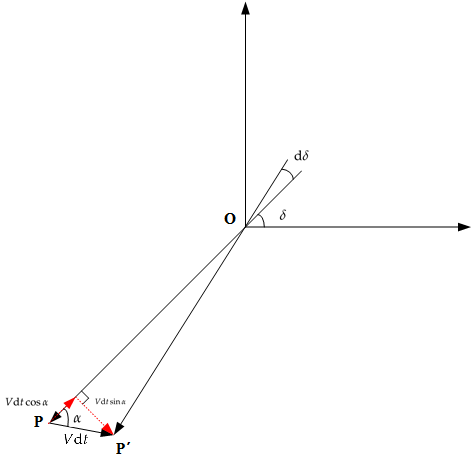
\includegraphics[width=0.5\textwidth]{RhoAlphaDelta2.png}
\caption{Polar Coordinates}
\label{RhoAlphaDeltaFigure2}
\end{figure}

$\dot{\delta}$ also comes from only the control input of $V$ because $\delta$ is only related to the position of the vehicle. Consider that the vehicle moves for an infinitesimal time period $\mathrm{d}t$. Displacement of the vehicle is $V\mathrm{d}t$. We can know expression of $\mathrm{d}t$ from the figure \ref{RhoAlphaDeltaFigure2} that
\begin{equation} \label{dotdelta}
\begin{split}
\rho \mathrm{d}\delta = V \mathrm{d}t \sin\alpha \\
\dot{\delta} = \frac{\mathrm{d}\delta}{\mathrm{d}t}=\frac{V \sin\alpha}{\rho}  \\
\end{split}
\end{equation}

Expression of $\dot{\alpha}$ can be directly derived from \eqref{xytheta}, \eqref{coordinate transformation} and \eqref{dotdelta}.
\begin{equation} \label{dotalpha}
\begin{split}
\dot{\alpha} &= \dot{\delta} - \dot{\theta} \\
\dot{\alpha} &=  \frac{\mathrm{d}\delta}{\mathrm{d}t}=\frac{V \sin\alpha}{\rho} - \omega \\
\end{split}
\end{equation}

Combination of \eqref{dotrho}, \eqref{dotdelta}) and \eqref{dotalpha} is the dynamic equations of the unicycle in polar coordinates.
\begin{equation} \label{dotRhoDeltaAlpha}
\begin{split}
\dot{\rho}(t) &= -V(t) \cos(\alpha(t)) \\
\dot{\alpha}(t) &= \frac{V(t) \sin(\alpha(t))}{\rho(t)} - \omega(t) \\
\dot{\delta}(t) &= \frac{V(t) \sin(\alpha(t))}{\rho(t)}  \\
\end{split}
\end{equation}

In order to achieve the goal posture, variables ($\rho$, $\alpha$, $\theta$) should all converge to zero.

% ----------------------End of Polar Coordinates and Example------------------------------------------------- %
\pagebreak
\subsection{Control Law}

For the unicycle problem proposed above, a suitable closed-loop control law is given by:
\begin{equation}
\begin{split}
V=k_1 cos(\alpha)
\\
\omega=k_2 \alpha + k_1 \frac{sin(\alpha)cos(\alpha)}{\alpha}(\alpha + k_3 \delta)
\end{split}
\end{equation}
These equations are chosen by selecting V and $\omega$ which result in the Lyapunov functions being negative semi-definite. It is possible to prove that when this is the case, the state variables will go to zero if the controller has been properly implemented.

A negative semi-definite form of the Lyapunov function is necessary because we want our Lyapunov function to always be decreasing in time, as this suggests that it is tending towards an equilibrium point rather than going further away. The key here is to consider the Lyapunov function as one form of "energy" of the system, which decreases to a minimum at equilibrium points.

A more detailed derivation for this result can be found in \cite{lyupanov}.


 % -------------------- Trajectory Tracking -------------------- %
\section{Trajectory Tracking}
A method for trajectory tracking consists in compromising closed-loop and open-loop control. In fact, open-loop control methods are more computationally feasible to find, yet as we have seen they are not robust. On the other hand, closed-loop solutions can be robust but are more complicated to find since the necessary conditions for optimality are partial differential equations, instead of ordinary differential equations in the open-loop case.

We can formulate a solution as:

\begin{equation} \label{constrained}
\begin{split}
\: \: &u^*(t) = u_d(t) + \pi(x(t), x(t)-u_d(t)) \\
\end{split}
\end{equation}

where $u_d(t)$ is a nominal trajectory found using open-loop control techniques. We use closed-loop control techniques to find $\pi(x(t), x(t)-u_d(t))$ that keeps our trajectory as close as possible to the nominal one.

There exists a certain number of choices of techniques for trajectory tracking, among which:

\begin{itemize}
  \item Geometric strategies: \\
  \\ An example is pursuit control. An example of strategy for the robot is to constantly try to chase a point on the desired trajectory. This method is effective, but it is difficult to provide theoretical guarantees.
  \item Linearization techniques: \\
  \\ They can be separated in two:
  \begin{enumerate}
    \item Inexact linearization: \\
    \\
    The dynamics of a system are usually non-linear. Yet, in the case of tracking, if we are close enough to the nominal trajectory then the relative dynamics can be linearized. The inexactness of this method comes from the fact that we only use the first terms of the relative dynamics' Taylor Series expansion to find a linear control law.
    \\
    \item Exact linearization: \\
    \\
    This method consists in cancelling the non-linearities from the system's dynamics, and developing a tracking control law from the resulting linear system. More precisely: \\
    \\
    - Let's consider the system dynamics: $\dot{x} = f(x) + u$, with $f$ non linear.\\
     - We can set a virtual control input $v$ so that $u = v - f(x)$. Then $v$ is linear, and we obtain $\dot{x} = v$. \\
     - We then design v so that x converges to the origin. Our actual control input is therefore $v - f(x)$. \\
     \\
     Not all systems admit this linearization. Even for those who do, one should be careful in using this method since it relies on the exactness of our non-linear model $f$. In fact, if $f$ differs consequently from the real system dynamics, the non-linearities are not cancelled with this method and the consequences of using the resulting control law could be disastrous.
  \end{enumerate}
  \item Optimization based techniques: \\
  \\
  This consists in posing the problem of trajectory tracking as an optimal control problem. These techniques are thoroughly studied in AA203.
\end{itemize}
 % ----------------- END of Trajectory Tracking ----------------- %

\begin{thebibliography}{9}
\bibitem{lyupanov}
Aicardi, Casalino, Bicchi, Balestrino.
\textit{Closed loop steering of unicycle like vehicles via Lyapunov techniques}.
IEEE, Genoa, Italy, 1995.


\bibitem{lyupanovproof}
Wang, Zhanshan, Liu, Zhenwei, Zheng, Chengde
\textit{Qualitative Analysis and Control of Complex Neural Networks with Delays}.
Springer-Verlag Berlin Heidelberg,  2016.


\bibitem{dflatness}
Richard M Murray, \textit{Optimization-based control}. California Institute of Technology CA, 2009.

\bibitem{optcontrol}
D. K. Kirk. \textit{Optimal Control Theory: An introduction}. Dover Publications, 2004.

\bibitem{bvpstandardform}
Ascher, U., \& Russell, R. D. \textit{Reformulation of boundary value problems into ``standard'' form}. SIAM review, 23(2), 238-254, 1981.

\bibitem{ee363notes}
Notes from ee363 at Stanford University
\textit{https://stanford.edu/class/ee363/lectures/lyap.pdf}

\end{thebibliography}

\subsubsection*{Contributors}
Winter 2019: [Your Names Here]
\\
Winter 2018: Joseph Lorenzetti, Kenneth Hoffmann, Oriana Peltzer, Zhe Huang, William Mangram
\end{document}
